\chapter{Tervezés}

Mivel korábban már több játékot is készítettem ami négyzetrács alapú térképet használ, most szerettem volna megismerni, hogy a hexagon alapú térképek, hogyan készülnek, ezért választottam a hexagont a programom térképének alapjául a szakdolgozatomhoz. Ehhez eltolásos koordináta-rendszert fogok használni a megjelenítésben és a tárolásban, mivel téglalap alakú térképet szeretnék használni és ehhez a megoldáshoz a fentebb említettek alapján ez tűnt célszerű döntésnek. Viszont mivel az eltolásos koordináta-rendszerben a számítások bonyolultabbak mint a többi ismertetett koordináta-rendszerben, ezért a számításokhoz a koordinátákat átalakítom a kocka koordináta-rendszerbeli megfelelőjére és azzal fogom elvégezni a számításokat, majd pedig visszaalakítom a tároláshoz és a megjelenítéshez. Az útkereső algoritmusok közül az A* -ra esett a választásom, mivel az adott esetben ez a leghatékonyabb.

\section{Stílus és modellek}

A játékban szereplő grafikai stílusként a low-poly irányzatot választottam. Ehhez kezdetben saját készítésű modelleket használtam de a fejlesztés végéhez közeledvén a modellek egyre komplexebbek kezdtek lenni és nehézkesebbé vált a különböző objektumok egységes kinézetének kialakítása is. Ebből kifolyólag az interneten kerestem további modelleket.
\newline
\newline A játék fejlesztése során 3D-s modelleket használtam, mert ezáltal lehetőség nyílt arra, hogy a térképet forgatni lehessen és különböző szemszögekből lehessen látni a történéseket. Úgy ítéltem meg, hogy ez több előnnyel járna mint amennyi plusz energiát követelne meg.
\newline
\newline A térkép hexagonokból épül fel és a hexagonháló egyik fő jellemzője az, hogy a háló szélein lévő hexagonok nem egy vonalba esnek. Ennek az előnyeit és hátrányait korábban a 3.2 fejezetben már taglaltam. Jelen esetben a már említett problémák nem okoznak gondot, mivel nem kell igazodni semmilyen körülhatároló objektumhoz.

\begin{center}
  \begin{tabular}{ | c | c | c | c | }
    \hline
     & Sivatag & Normál & Havas \\ \hline
    Kisebb növények / kövek & 14 & 6 & 0 \\ \hline
    Fák & 4 & 4 & 4 \\ \hline
    Épületek & 6 & 6 & 6 \\ \hline
    Hegyek & 2 & 2 & 2 \\ \hline
  \end{tabular}
\end{center}

\section{Kamera}

A programban izometrikus kamerát használok. Ez a megoldás gyakori a stratégiai játékoknál. A legtöbb számítógépes játék esetében az izometrikus nézet nem fedi a matematikai értelemben vett izometrikus nézetet ($\textasciitilde 35$ fok). Gyakran előfordul 30, 45, 53, 60 fokos kamera is. Ezek közül talán a legérdekesebb az 53 fok, ami a régebbi kijelzőknek a felbontásának arányából (4:3) adódott. 

$$
atan(4 / 3) = 53.1301024 \space deg
$$

\noindent Ezek közül a 45 és a 60 fokos megoldás nyújtotta azt a hatást amit szerettem volna, végül a 45 fokos szög mellett döntöttem a laposabb szög miatt. Ehhez 60 fokos látószöget (FOV) alkalmaztam. A kamera körbeforgatható a horizontális tengely körül 360 fokban, ezt a 3D-s modellek miatt van lehetőség megoldani, ezáltal van lehetőség több szempontból megvizsgálni a térképen az objektumok elhelyezkedését. Lehetőség van arra, hogy a térképre ráközelítsünk vagy távolodjunk tőle, ennek megvan a felső és alsó határa. Igyekeztem úgy megválasztani ezeket a határokat, hogy ne lehessen túl közel vagy túl távol vinni a kamerát a térképtől, mindazonáltal ez a funkció még betudja tölteni a szerepét. A kamera természetesen a térkép mentén mozgatható mind a 4 irányban. 
\newline
\newline A játékfejlesztésben az egyik legnehezebb feladat a kamera kezelés megvalósítása, mivel ha jól működik senki sem veszi észre, ha pedig hibásan működik akkor a teljes felhasználói élményt tönkreteheti. Ezért úgy döntöttem, hogy egy olyan kódot használok fel a Unity store-ból amit már korábban is használtam és kisebb módosítások alkalmazásával minden szempontot megvalósít.

\section{Generálás lépései}

Bemenetként a térkép fő jellemzőit, a generált térképpel szembeni elvárásokat kapja paraméterezésként a program. Bizonyos paraméterek szabályozhatóak a generálás után is (“hőmérséklet”), de a többségük nem. A térképnek a főbb paraméterei szabályozhatóak: méret, környezeti viszonyok, domborzat, folyók, növényzet, épületek. Egyéb apró paraméterei nem módosíthatóak a játék használta közben, de a Unity szerkesztőben (Unity editor) az Inspector ablakokban a többségük állítható. Ezt azért alakítottam így ki mert nem akartam a felhasználói felületet túl komplikálttá tenni inkább az egyszerűségre törekedtem. Az Inspector ablakon lehetséges módosítani a mesh-eket, textúrákat, shadereket, konstansokat.
\newline
\newline A térkép egy több lépcsős folyamat végén fog elkészülni. Ezeket a lépéseket a következő pontban fogom bemutatni.

\noindent Első lépésként szükségünk lesz egy csempére (tile), ami az alapelem lesz a térképen. Erre a célra én egy 3D-s hexagon modellt használtam különböző textúrákkal. A különböző textúrák és a modellek csak a Unity-n belül egy úgynevezett Inspector panelen módosíthatóak. A játékban jelenleg a hexagonhoz 6 különböző textúra szerepel (fű, homok, hó, víz, jég, óceán (térkép széle)).
\newline
\newline Ezen kívül szükség van a generálni kívánt térkép méreteire (szélesség, magasság). Ezek a paraméterek a generálás előtt a felhasználó által is szabályozhatóak bizonyos keretek között.

\subsection{Térkép széle}

A térkép körülhatárolására egy speciális hexagon textúrát hoztam létre ami az óceánt szimbolizálná. Ez gyakori megközelítés a stratégiai játékok esetén a térkép körülhatárolására (pl: \textit{Civilization IV: Colonization}). A játékfejlesztők különböző módszerekkel határolják körbe a térképet: felhők, hegyek, várfalak, óceánok, stb. A lényege, hogy a karakterek ne tudjanak a széleket határoló néhány mezőre lépni. Fontos még, hogy valami speciális mező legyen.
\newline
\newline A beállított magasság és szélesség értékeken felül fog az algoritmus minden egyes szélre egy plusz sort generálni a széleknek, ezáltal, ha a felhasználó a térkép méreteit $x \times y$ -nak adta meg a kapott térkép mérete $(x+2) \times (y+2)$ méretű lesz.

\subsection{Domborzat}

A második elem ami majd a térképen meghatározásra kerül az a domborzat, mely két fajta magasságban jelenik majd meg (domb, hegy), ehhez két különböző modellt fog használni. A térkép méreteihez viszonyítva lehet majd százalékos arányban kifejezni a domborzat mennyiséget, egy $0\%$-tól $40\%$-ig terjedő skálán. Ezt az intervallumot találtam megfelelőnek ahhoz, hogy ha sok hegyek akarunk akkor sok hegyet kapjunk de még a karakterek által bejárható maradhasson a térkép. Ezt az intervallumot a generálás előtt áll majd módjában a felhasználónak beállítani. A hegyek és a dombok véletlenszerű pozícióban fognak elhelyezkedni. A különböző környezeti viszonyokhoz három különböző textúra áll rendelkezésre (fű, homok, hó). A hegyek és a dombok eloszlása teljesen véletlenszerűen lesz kialakítva és nincs beleszólása a felhasználónak.

\subsection{Folyók}

A folyók generálásakor két különböző esetet különböztettem meg. Amikor vannak hegyek és amikor nincsenek. Amikor vannak hegyek akkor az egyik hegy lábától egy másik vizes mezőig (a térkép szélei vagy egy már meglévő folyó) generál az algoritmus folyó egy útkereső algoritmus felhasználásával. Abban az esetben amikor nincs egy darab hegy sem akkor az algoritmus vagy véletlenszerűen választ egy mezőt a térképen és egy vizes mezőig generál. A domborzathoz hasonlóan a vizes mezők mértéke is szabályozható a felhasználó által a generálás előtt. Ez is a domborzatnál már megismert $0\%$-tól $40\%$-ig tartó skálán mozog a térkép méretéhez viszonyítva. A környezeti viszonyokhoz alkalmazkodva kétfajta textúra jöhet szóba: normál és jeges. Ez a módszer viszonylag könnyen implementálható az útkereső algoritmus ismeretében és kellően egyedi megjelenést tud kölcsönözni a térképnek. Keletkezhetnek szigetek, szélesebb folyók, torkolatok. Ezen kívül minden vizes mező hozzáadódik egy listához aminek majd a vízszint meghatározásában lesz szerepe.

\begin{figure}[h!]
\centering
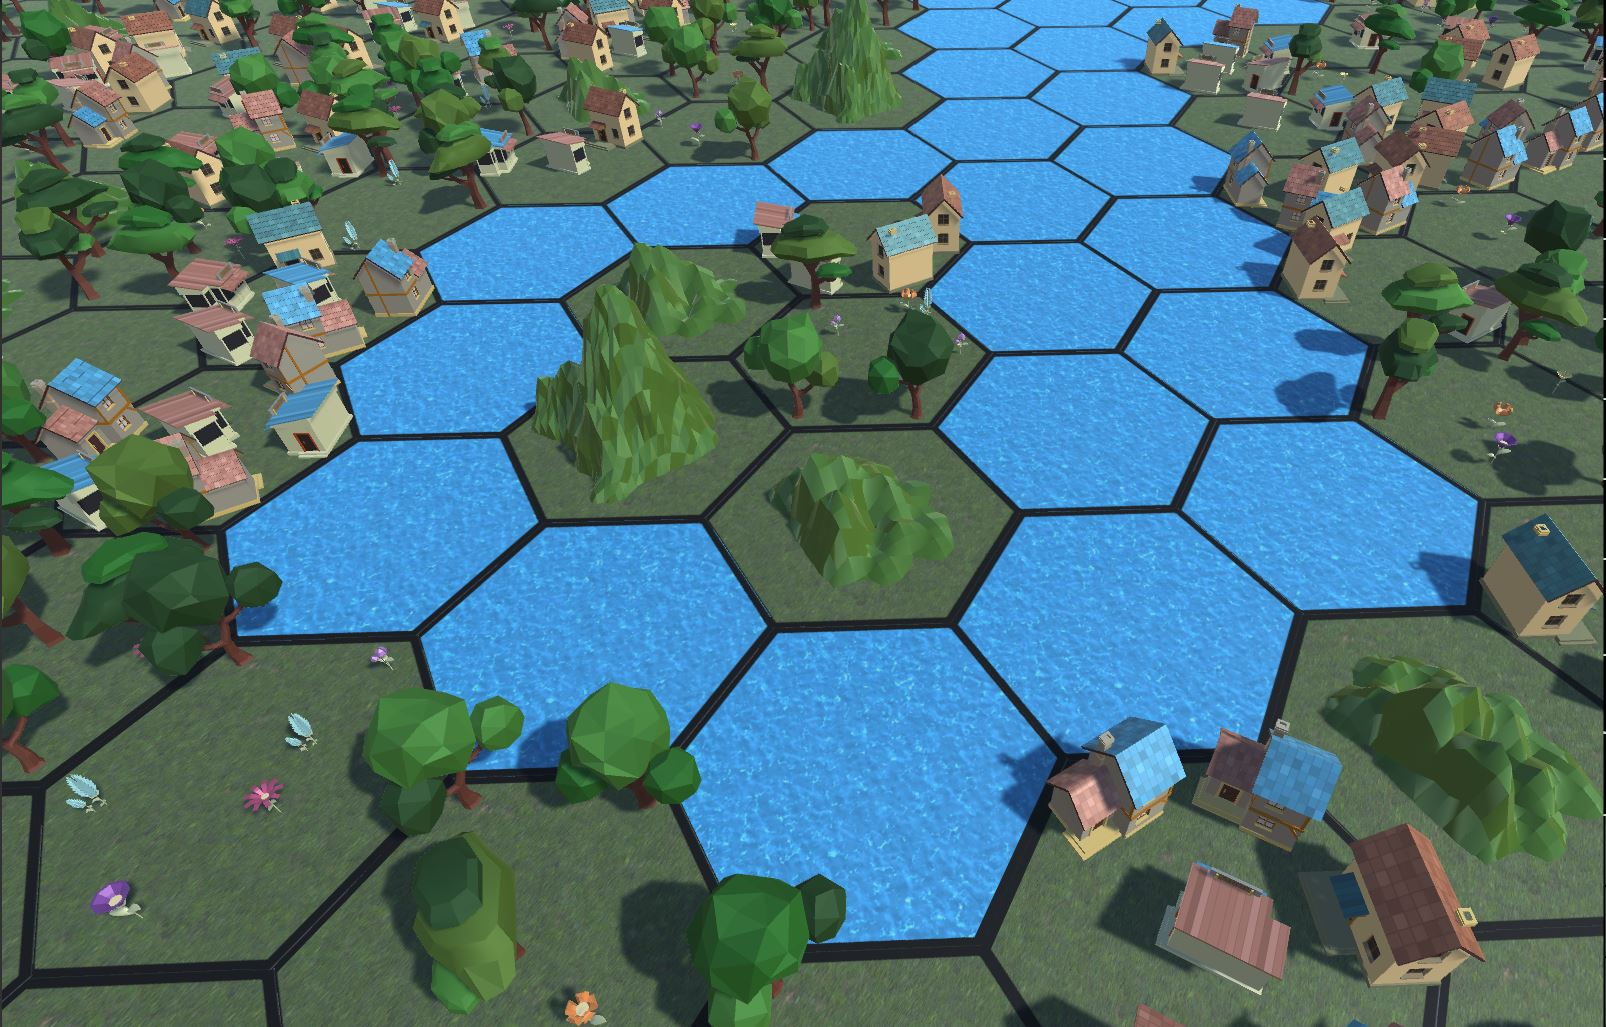
\includegraphics[scale=0.3]{kepek/Island.JPG}
\caption{Sziget}
\label{fig:Island}
\end{figure}

\begin{figure}[h!]
\centering
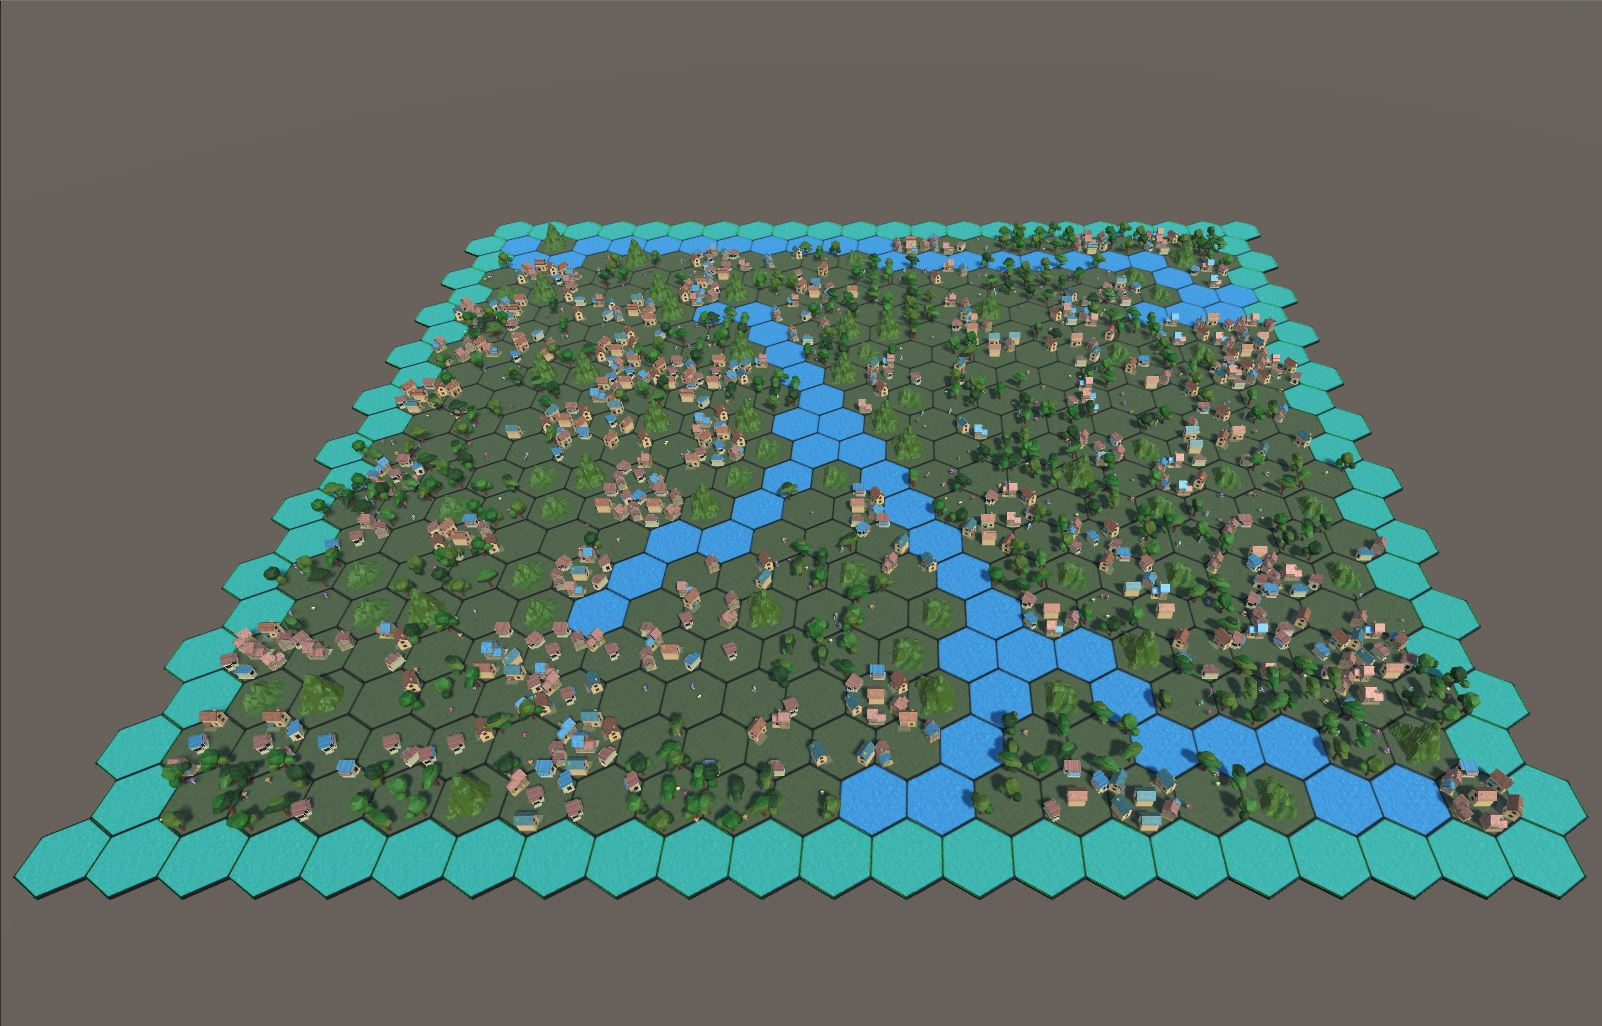
\includegraphics[scale=0.3]{kepek/Branch.JPG}
\caption{Elágazások a folyón}
\label{fig:Branch}
\end{figure}

\subsection{Sík területek generálása}

Az algoritmus minden olyan mezőre ahová még nem generált domborzatot vagy folyót oda sík terültet fog generálni. Ezek sima hexagonokból fognak állni és a további paraméterek segítségével kerülhetnek majd erre épületek, fák, virágok. Itt is a már megszokott 3 textúra áll majd rendelkezésre (fű, homok, jég).

\subsection{Vízszint meghatározása}

A vízszint meghatározása minden mezőre a növényzet generálásához szükséges. A vízszint a vizes mezőktől távolodva lineárisan csökken. Ezáltal megvalósítható, hogy minél távolabb van egy mező a víztől annál kisebb az esélye, hogy sok növényzet legyen rajta. A hőmérséklet mellett még a vízszint fog közrejátszani abban, hogy hogyan száradjanak ki a különböző mezők.

\subsection{Épületek}

Úgy terveztem, hogy az épületek és a fák 7 fix pozícióban állhatnak a hexagonon. Azért döntöttem a 7 fix pont mellett mert így egyszerűbb lehet az algoritmus mintha véletlenszerű pozíciókban szerepelnének a hexagonon. Így nem kell vizsgálni, hogy az objektumok amiket elhelyezne az algoritmus azok ütköznek-e valamilyen egyéb objektummal a térképen. Mindössze csak arra kell figyelni, hogy egy helyen csak egy objektumot tudjunk elhelyezni. A további fejlesztések esetén például az úthálózatot is könnyebben megvalósíthatónak tartom mintha véletlenszerű helyeken lennének és nem is feltétlenül lenne jobb megoldás. Kétfajta épület van. A házak esetén a környezeti változások a falakat nem, csak a háztetők textúráját érinti (normál, hó).

\begin{figure}[h!]
\centering
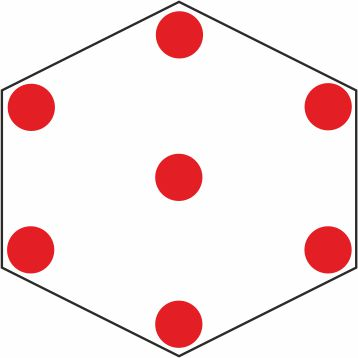
\includegraphics[scale=1]{kepek/Places.jpg}
\caption{Az épületek és fák elhelyezkedési pontjai a hexagonon}
\label{fig:Places}
\end{figure}

\begin{figure}[h!]
\centering
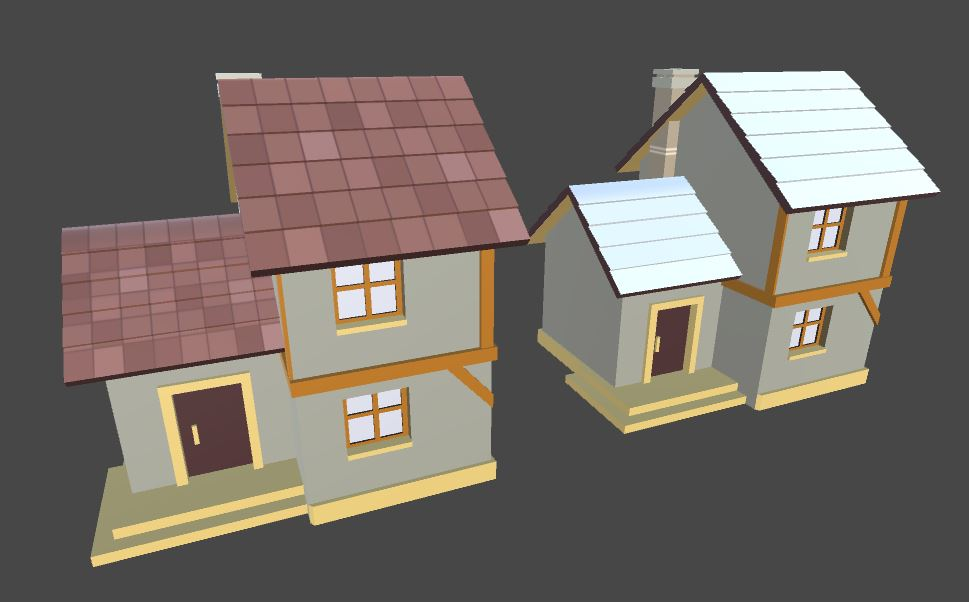
\includegraphics[scale=0.3]{kepek/Buildings.JPG}
\caption[épület]{Egy épület normál körülmények között (bal oldal) és havas körülmények között (jobb oldal). \footnotemark}
\label{fig:Buildings}
\end{figure}

\footnotetext{www.assetstore.unity3d.com/en/\#!/content/50095}

\subsection{Növényzet}

A növényzetet úgy tervezem megvalósítani, hogy két csoportra bontom azt. Az egyik a fák, a másik pedig a kisebb objektumok pl: virágok, kaktuszok, kövek.  Mind a két csoportot másképpen valósítottam meg.

\subsubsection{Fák}

Az épületeknél már megismert módszerrel 7 fix helyre kerülhetnek egy mezőn belül. Két különböző modell fog szerepelni a játékban az időjárási viszonyoknak megfelelően pedig három különböző módon jelenhetnek majd meg. A különböző viszonyoknak megfelelően fog különböző szinekből generálni a fáknak lomb színt az algoritmus, ezt egy listán lehet majd megadni a különböző esetekhez. A fák csak sík mezőkön generálódhatnak majd, ezáltal egyszerűsítve a generálást.

\begin{figure}[h!]
\centering
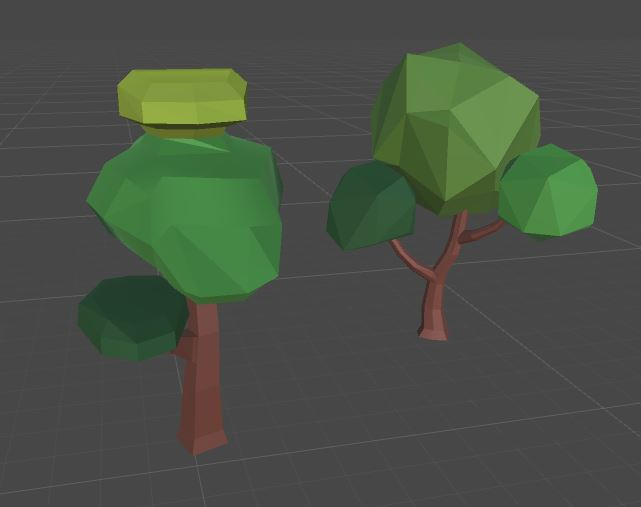
\includegraphics[scale=0.32]{kepek/Tree_Normal.JPG}
\caption[normal]{Normál esetben a fák lombja a zöld különböző árnyalataiból állhat. \footnotemark}
\label{fig:Tree_Normal}
\end{figure}

\footnotetext{www.assetstore.unity3d.com/en/\#!/content/52217}

\begin{figure}[h!]
\centering
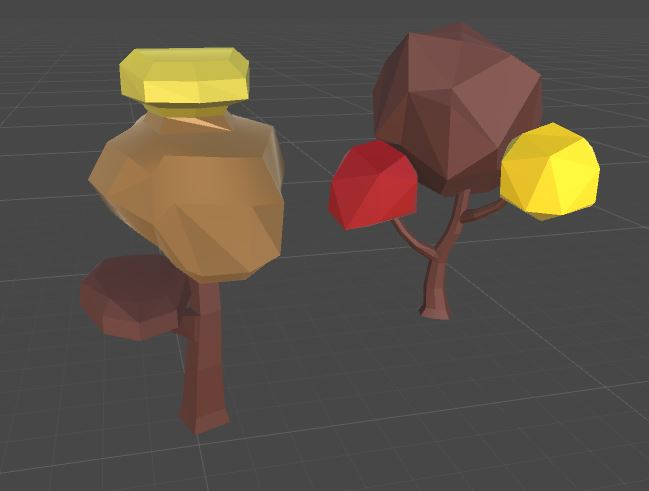
\includegraphics[scale=0.32]{kepek/Tree_Fall.JPG}
\caption[Ősz]{“Ősz” A lomb színei ebben az esetben több különböző szín árnyalatából tevődik össze (piros, barna, sárga). \footnotemark}
\label{fig:Tree_Fall}
\end{figure}

\footnotetext{www.assetstore.unity3d.com/en/\#!/content/52217}

\begin{figure}[h!]
\centering
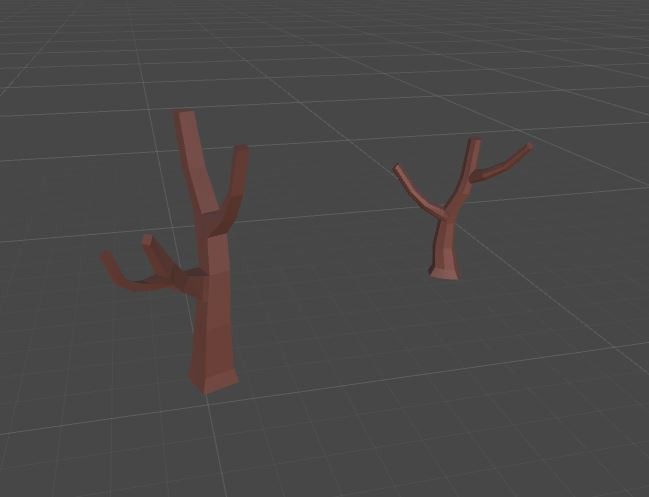
\includegraphics[scale=0.32]{kepek/Tree_Winter.JPG}
\caption[tél]{Kiszáradt vagy jeges Ebben az esetben mint látható az algoritmus elrejti a lombokat. \footnotemark}
\label{fig:Tree_Winter}
\end{figure}

\footnotetext{www.assetstore.unity3d.com/en/\#!/content/52217}

\newpage
\subsubsection{Kisebb objektumok}

Véletlenszerű pozíciókban fogja majd generálni az algoritmus a sík mezőkön. A kisebb objektumok közé tartoznak a virágok, kaktuszok, kövek. A kaktuszok és a kövek a homokos területeken, míg a virágok a füves területeken fordulnak elő. 

\begin{figure}[h!]
\centering
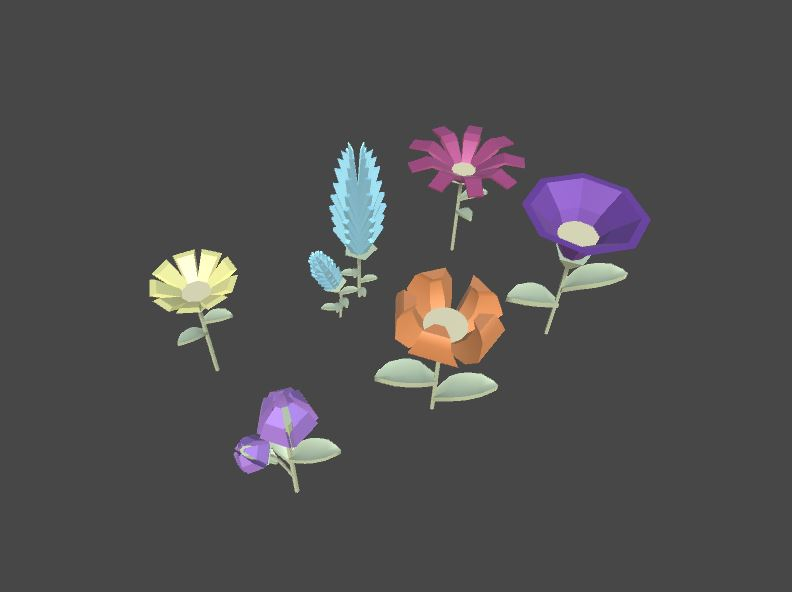
\includegraphics[scale=0.4]{kepek/Flowers.JPG}
\caption[Virágok]{Virágok \footnotemark}
\label{fig:Flowers}
\end{figure}

\footnotetext{www.assetstore.unity3d.com/en/\#!/content/47083}

\begin{figure}[h!]
\centering
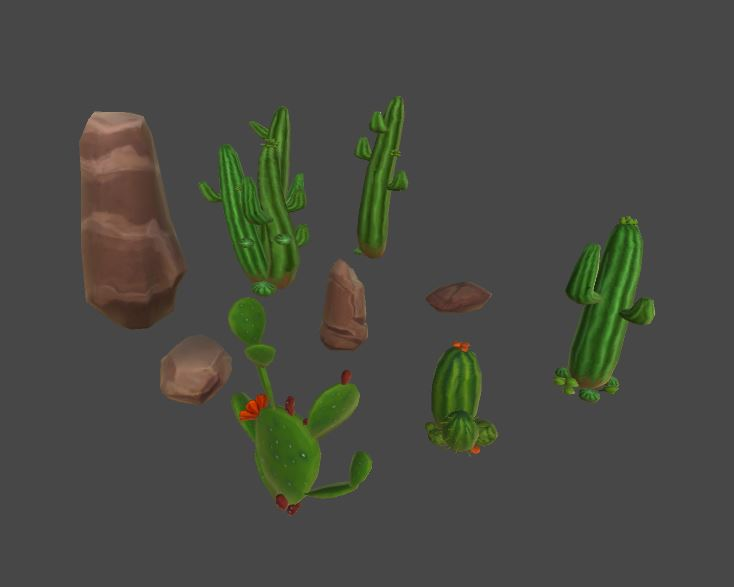
\includegraphics[scale=0.4]{kepek/Cactus.JPG}
\caption[Kaktuszok és kövek]{Kaktuszok és kövek \footnotemark} 
\label{fig:Cactus}
\end{figure}

\footnotetext{www.assetstore.unity3d.com/en/\#!/content/11547}

\subsection{Hőmérséklet}

Lehetőség lesz az évszakok között váltogatni, ez a funkció fontos a játék tovább fejlesztésével kapcsolatban, mivel a játékban szerepet kap majd az évszakok változása. A tavasz és az ősz nem változtatja az alap hőmérsékleti viszonyokat csak a nyár és a tél módosítja a globális hőmérsékletet egy konstans értékkel. 
\newline
\newline A különböző objektumokra a térképen elfoglalt helyük alapján és egyéb tulajdonságaik miatt különböző módon hat majd az időjárás. Ezt próbálom meg most lépésről lépésre bemutatni.
\newline
\newline Elsődlegesen egy globális hőmérséklet paramétert készítek ami minden egyes mezőre egységes mértékben vonatkozik és a többi paraméter pedig ehhez adódik hozzá. Ezzel már lesz lehetőség a különböző ''évszakokat'' tesztelni a játékban. Amikor a különböző grafikai elemek is elkészülnek, akkor kezd el a további paramétereket hozzáadni.
\newline
\newline Ekkor úgy egészítem ki az algoritmust, hogy a térkép “teteje” és “alja” között lehetséges legyen egy átmenetet megvalósítani, mintha egy nagyobb kontinens lenne. Ennek a paraméternek lehetséges negatív és pozitív értéket is megadni, amelyek azt befolyásolják, hogy milyen mértékben fog növekedni vagy csökkenni a hőmérséklet mezőről mezőre.

\begin{figure}[h!]
\centering
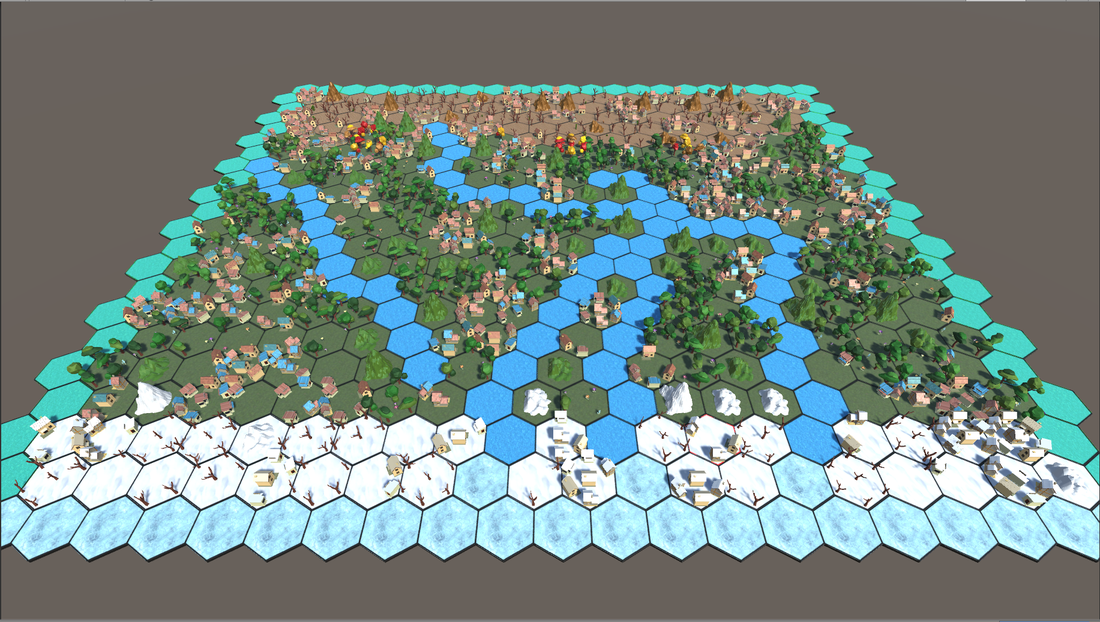
\includegraphics[scale=0.5]{kepek/transition.png}
\caption{Hőmérséklet átmenet}
\label{fig:transition}
\end{figure}

\noindent Majd pedig egy olyan paramétert készítek amivel dinamikusan lehet a generált térképen változtatni a hőmérsékletet. Ez is változtatható pozitív és negatív értékűre annak függvényében, hogy “melegebb” vagy hidegebb környezetet szeretnénk elérni.
\newline
\newline Végezetül a különböző objektumok tulajdonságaival fogok foglalkozni. Ezalatt azt értem, hogy a vizes mezők alacsonyabb hőmérséklet mellett kezdenek el “befagyni” mint a sík mezők vagy azok a mezők hamarabb kezdenek el kiszáradni, ahol kevesebb a víz.

